


% =============================================================================
% ================================================================ Header Stuff
% =============================================================================

\documentclass{beamer}
\usepackage[utf8]{inputenc}
\usepackage{epsfig} % Allows the inclusion of eps files
\usepackage{epic} % Enhanced picture mode
\usepackage{eepic} % Extensions for epic
\usepackage{units} % SI unit typesetting
\usepackage{url} % URL handling
\usepackage{longtable} % Tables that continue onto multiple pages
\usepackage{mathrsfs} % Support for \mathscr script
\usepackage{multirow} % Span rows in tables
\usepackage{amssymb} % AMS math symbols and helpers
\usepackage{graphicx} % Enhanced graphics support
\usepackage{setspace} % Adjust spacing in captions, single by default
\usepackage{xspace} % Automatically adjusting space after macros
\usepackage{amsmath} % \text, and other math formatting options
\usepackage{siunitx} % \num{} formatting and SI unit formatting
\usepackage{booktabs} % Enhanced tables with \toprule, etc.
\usepackage{hyperref} % Add clickable links to other parts of the document
\usepackage[noabbrev,capitalize]{cleveref} % Automatically determine \cref type
\usepackage[hang,flushmargin]{footmisc} % Prevent indent in footnotes. 
\usepackage{xcolor} % so we can put todo notes in color. 
\usepackage{parskip} % http://ctan.org/pkg/parskip vskip instead of indent. 
\usepackage{float} % Sometimes you want to tell LaTeX to put an image RIGHT HERE. 
% Prevent LaTeX from putting a figure right before the start of a section. 
\usepackage[section]{placeins}
\usepackage[percent]{overpic}



\usepackage{empheq}
\usepackage{tcolorbox}


% Try to prevent widows and orphans -- dangling parts of paragraphs over page breaks. 
\widowpenalty10000
\clubpenalty10000
% Configure the siunitx package
\sisetup{
    group-separator = {,}, % Use , to separate groups of digits, like 12,345
    list-final-separator = {, and } % Always use the serial comma in \SIlist
}
% Configure the cleveref package
\newcommand{\creflastconjunction}{, and } % Always use the serial comma



% Names with special characters. 
\newcommand{\Alfven}{Alfv\'en\xspace}
\newcommand{\Ampere}{Amp\`ere\xspace}

% To make sure the capitalization is consistent. 
\newcommand{\ohmlaw}{Ohm's Law\xspace}
\newcommand{\amplaw}{\Ampere's Law\xspace}
\newcommand{\farlaw}{Faraday's Law\xspace}

% Field-aligned unit vectors. 
\newcommand{\xhat}{\ensuremath{\hat{x}}\xspace}
\newcommand{\yhat}{\ensuremath{\hat{y}}\xspace}
\newcommand{\zhat}{\ensuremath{\hat{z}}\xspace}

% Spherical unit vectors. 
\newcommand{\rhat}{\ensuremath{\hat{r}}\xspace}
\newcommand{\qhat}{\ensuremath{\hat{\theta}}\xspace}
\newcommand{\fhat}{\ensuremath{\hat{\phi}}\xspace}

% Use underlines for vectors and tensors. 
\renewcommand{\vec}[1]{\underline{#1}}
\newcommand{\tensor}[1]{\underline{\underline{#1}}}

% Differential operators. 
\newcommand{\dd}[1]{\ensuremath{ \frac{\partial}{\partial #1} }\xspace}
\newcommand{\ddt}{\dd{t}\xspace}
\newcommand{\curl}[1]{\ensuremath{ \nabla \times \vec{#1} }\xspace}
\renewcommand{\div}[1]{\ensuremath{ \nabla \cdot \vec{#1} }\xspace}
\newcommand{\grad}[1]{\ensuremath{ \nabla #1 }\xspace}

% Properly-scaled parentheses for grouping terms or for arguments. 
\newcommand{\lr}[1]{ \left( #1 \right) }
\newcommand{\lrsmall}[1]{ \left( {\scriptstyle #1} \right) }
\renewcommand{\arg}[1]{\!\lr{#1}}
\newcommand{\argsmall}[1]{\!\lrsmall{#1}}
\newcommand{\lrb}[1]{ \left[ #1 \right] }

% Circled plus-minus symbol. Solving quartics requires \pm and \opm. 
\newcommand{\opm}{ \text{ \textcircled{ \ensuremath{\hskip -0.2em \pm} } } \xspace}

% Define a better looking eV by moving the V slightly left
\DeclareSIUnit\electronvolt{e\hspace{-0.08em}V}

\DeclareSIUnit\RE{R_E}


\newcommand{\dt}{\ensuremath{\delta \hspace{-0.1em} t} \xspace}



% Azimuthal modenumber, typically indicated with a lowercase m. 
\newcommand{\azm}{\ensuremath{m_{azimuthal}}\xspace}

% Azimuthal modenumber, typically indicated with a lowercase m. 
\newcommand{\me}{\ensuremath{m_{e}}\xspace}

% Jacobian dererminant, typically indicated with a capital J, which we are using for current. 
\newcommand{\jac}{\ensuremath{D}\xspace}

% Dispersion tensor, typically indicated with... a capital D?
\newcommand{\dispersiontensor}{\tensor{T}\xspace}


% These things just get used a lot in the dispersion relation chapter...

% Boris-corrected speed of light. 
\newcommand{\cb}{\ensuremath{c_B} \xspace}

% Boris-corrected plasma frequency. 
\newcommand{\ob}{\ensuremath{\omega_B} \xspace}

% Boris-corrected electric constant. 
\newcommand{\eb}{\ensuremath{\epsilon_B} \xspace}

% Alfven speed. 
\newcommand{\va}{\ensuremath{v_A} \xspace}

% Perpendicular electric constant. 
\newcommand{\ep}{\ensuremath{\epsilon_\bot} \xspace}

% Epsilon zero. 
\newcommand{\ez}{\ensuremath{\epsilon_0} \xspace}

% Conductivities. 
\newcommand{\sz}{\ensuremath{\sigma_0} \xspace}
\newcommand{\sh}{\ensuremath{\sigma_H} \xspace}
\renewcommand{\sp}{\ensuremath{\sigma_P} \xspace}




\newcommand{\spe}{\ensuremath{\frac{\sigma_P}{\ep}} \xspace}
\newcommand{\she}{\ensuremath{\frac{\sigma_H}{\ep}} \xspace}




% 3x3 matrix. 
\newcommand{\mmm}[9]{ \left[ \begin{array}{ccc}
    #1 & #2 & #3 \\
    #4 & #5 & #6 \\
    #7 & #8 & #9
  \end{array} \right] }

% 2x2 matrix. 
\newcommand{\mm}[4]{ \left[ \begin{array}{cc}
    #1 & #2 \\
    #3 & #4
  \end{array} \right] }

% 2x1 matrix, or 2-vector. 
\newcommand{\vv}[2]{ \left[ \begin{array}{c}
    #1 \\
    #2
  \end{array} \right] }


% Physics constants
\newcommand{\C}{{\mathrm{c}}}

% Add space between rows of tables
\newcommand{\spacerows}[1]{\renewcommand{\arraystretch}{#1}}









\AtBeginSection[]{
  \begin{frame}
  \vfill
  \centering
  \begin{beamercolorbox}[sep=8pt,center,shadow=true,rounded=true]{title}
    \usebeamerfont{title}\insertsectionhead\par%
  \end{beamercolorbox}
  \vfill
  \end{frame}
}




\usepackage{beamerthemesplit}

\newcommand{\backupbegin}{
   \newcounter{finalframe}
   \setcounter{finalframe}{\value{framenumber}}
}
\newcommand{\backupend}{
   \setcounter{framenumber}{\value{finalframe}}
}

% =============================================================================
% ============================================================== Begin Document
% =============================================================================

\title[FLR in 2.5D]{Field Line Resonance in ``Tuna Half'' Dimensions}
%\subtitle{PhD Defense}
%\institute{University of Minnesota}
\author{Charles McEachern}
\date{28 April 2016}

\usetheme{Boadilla}
\usefonttheme{serif}

\begin{document}

% =============================================================================
% ================================================================= Title Slide
% =============================================================================

\frame{\titlepage}

% =============================================================================
% ================================================================ Introduction
% =============================================================================

\section{Introduction}

% -----------------------------------------------------------------------------
% -----------------------------------------------------------------------------
% -----------------------------------------------------------------------------

\begin{frame}
\frametitle{Earth's Magnetic Field}

When shaken by the solar wind, etc, Earth's magnetic field lines rattle. 

\vfill

\begin{overpic}[width=0.6885\textwidth]{figures/nasa_magnetosphere.jpg}
 \put (0, 1) {\tiny\textcolor{white}{\;NASA}}
\end{overpic}%
\begin{overpic}[width=0.3115\textwidth]{figures/flora_borsi.jpg}
 \put (0, 1) {\tiny\textcolor{white}{\;Fl{\'o}ra Borsi}}
\end{overpic}%

\end{frame}

% -----------------------------------------------------------------------------
% -----------------------------------------------------------------------------
% -----------------------------------------------------------------------------

\begin{frame}
\frametitle{\Alfven Waves}

\begin{columns}
\column{0.5\textwidth}
\begin{wideitemize}
\item Shear \Alfven waves carry energy along magnetic field lines. 
\item Compressional \Alfven waves can carry energy across field lines. 
\item A field line resonance (FLR) is a shear \Alfven wave that fills the field line exactly. 
\end{wideitemize}
\column{0.5\textwidth}
\begin{overpic}[width=\textwidth]{figures/kv_alfven.png}
 \put (0, 1) {\tiny\textcolor{black}{\;Kivelson and Russell}}
\end{overpic}%
\end{columns}

\end{frame}

% -----------------------------------------------------------------------------
% -----------------------------------------------------------------------------
% -----------------------------------------------------------------------------

\begin{frame}
\frametitle{Characterizing Field Line Resonances}

\vfill

Three properties by which FLRs can be characterized:
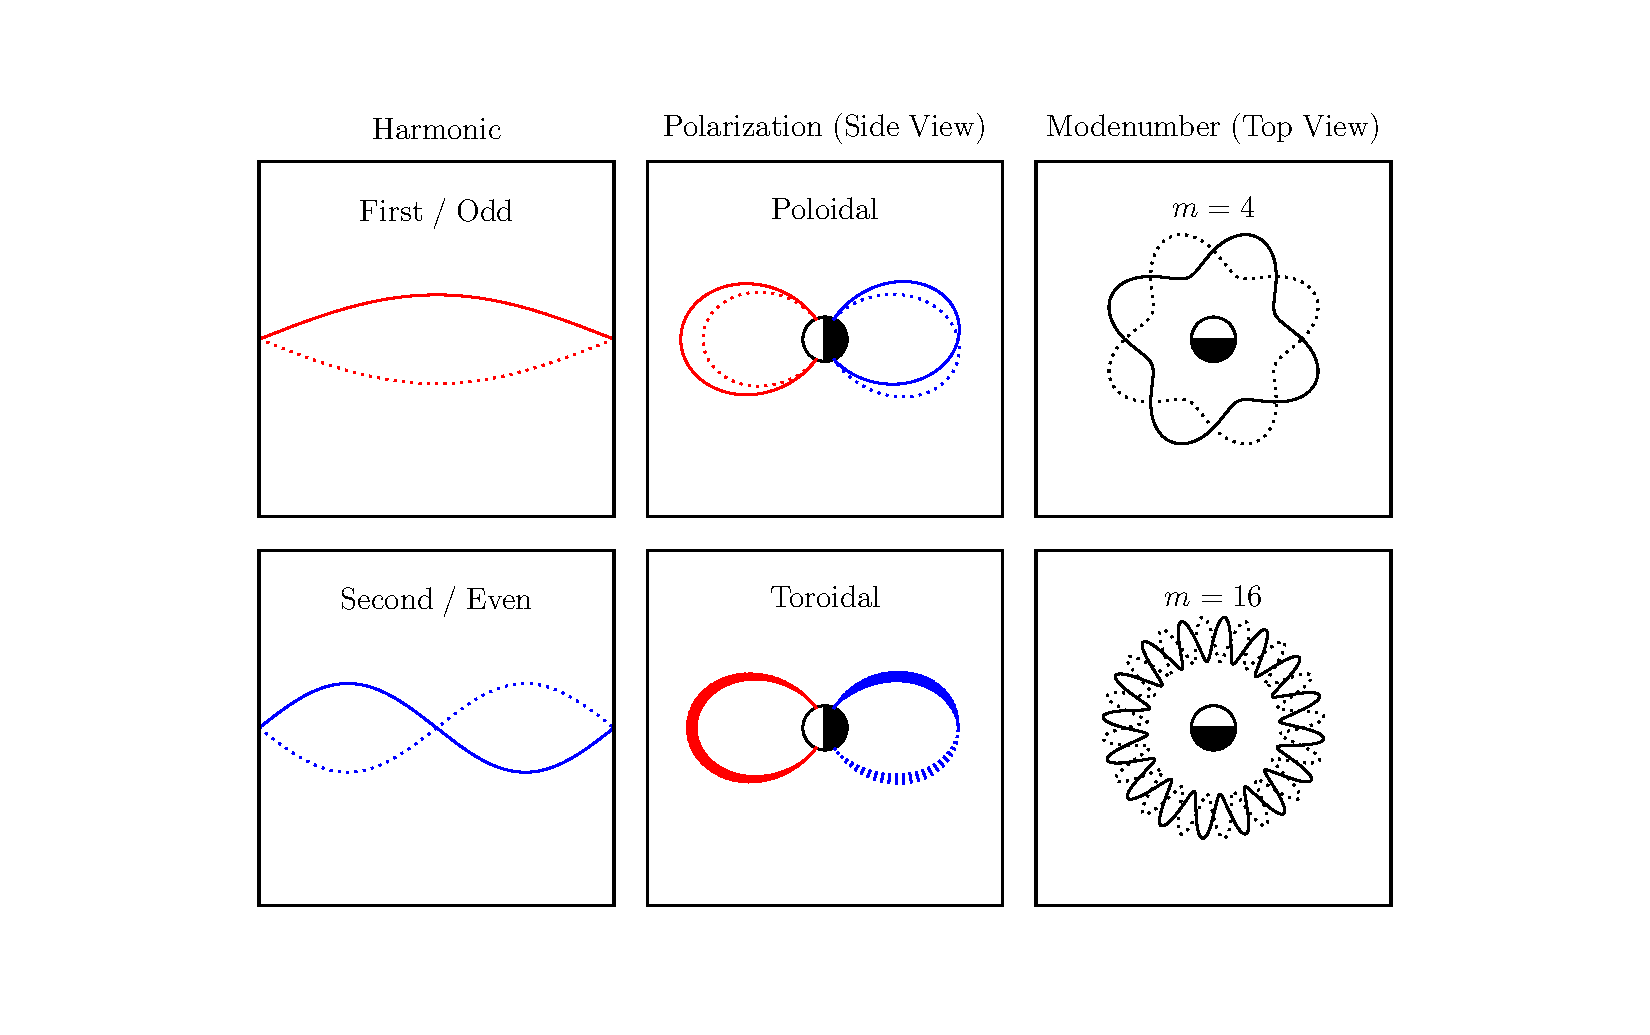
\includegraphics[width=\textwidth]{figures/properties.pdf}

\end{frame}

% -----------------------------------------------------------------------------
% -----------------------------------------------------------------------------
% -----------------------------------------------------------------------------

\begin{frame}
\frametitle{Pc4s and Giant Pulsations}

\begin{wideitemize}
\item Pc4 pulsations (\SIrange{7}{22}{\mHz}) resonate at auroral latitudes. 
\item They interact with trapped energetic particles. 
\item Giant pulsations are a small, distinctive subset of Pc4s.  
\end{wideitemize}

\vfill

\begin{center}
IAGA Frequency Bands [Jacobs, 1964]
\begin{tabular}{ @{\extracolsep{\fill}} cccccc @{\extracolsep{\fill}} }
  \hline
  & Pc1 & Pc2 & Pc3 & Pc4 & Pc5 \\
  \hline
  Period (\si{\second}) & 0.2--5    & 5--10    & 10--45  & 45--150 & 150--600 \\
  Frequency (\si{\mHz}) & 200--5000 & 100--200 & 22--100 & 7--22   & 2--7     \\
  \hline
\end{tabular}
\end{center}

\end{frame}

% =============================================================================
% ======================================================================= Model
% =============================================================================

\section{Numerical Model}

% -----------------------------------------------------------------------------
% -----------------------------------------------------------------------------
% -----------------------------------------------------------------------------

\begin{frame}
\frametitle{``Tuna Half'' Dimensional Grid}

\begin{columns}
\column{0.5\textwidth}
\begin{wideitemize}
\item Near Earth, at high \azm, 3D is too expensive. 
\item Earthward boundary is important for Pc4s --- keep it realistic. 
\item Simplifying assumption: everything goes as $\exp\arg{i \azm \phi}$. 
\item Grid is 2D, but fields and curls are 3D vectors. 
\end{wideitemize}
\column{0.5\textwidth}
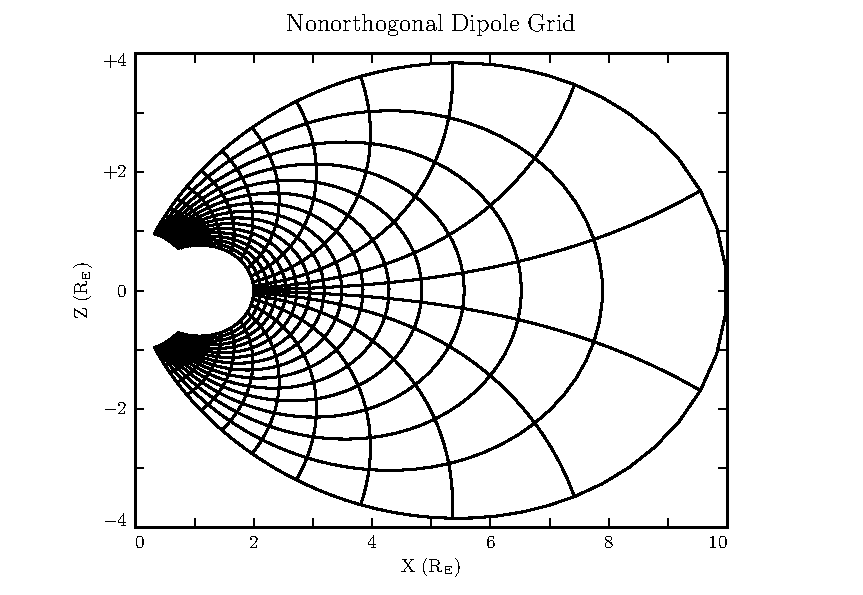
\includegraphics[width=\textwidth]{figures/grid.pdf}
\end{columns}

\end{frame}

% -----------------------------------------------------------------------------
% -----------------------------------------------------------------------------
% -----------------------------------------------------------------------------

\begin{frame}
\frametitle{Physical Parameter Profiles}

\begin{wideitemize}
\item Height-resolved conductivity from Kelley, modified by Lysak. 
\item Plasma density, including the plasmasphere. 
\item Four profiles: active day, quiet day, active night, quiet night. 
\end{wideitemize}

\vfill

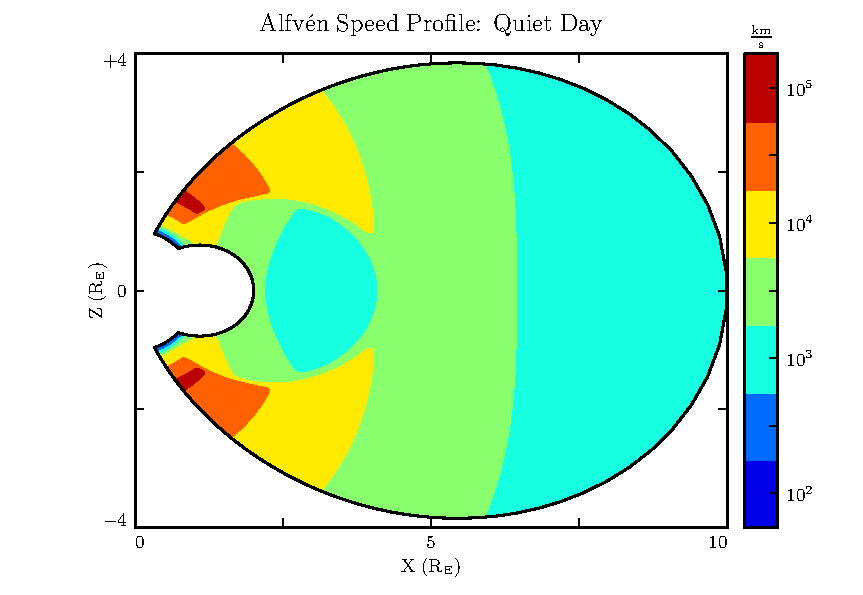
\includegraphics[width=0.5\textwidth]{figures/va_2.pdf}%
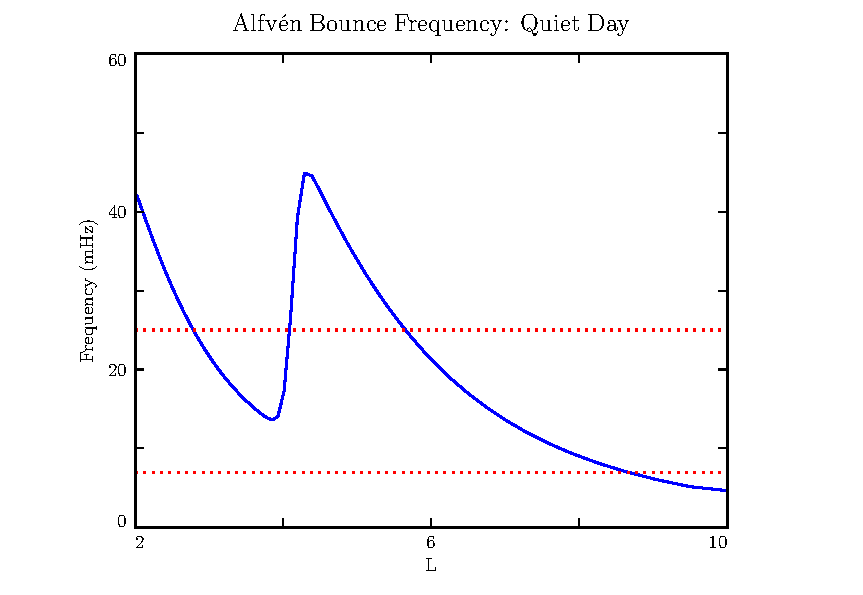
\includegraphics[width=0.5\textwidth]{figures/fa_2.pdf}%

\end{frame}

% -----------------------------------------------------------------------------
% -----------------------------------------------------------------------------
% -----------------------------------------------------------------------------

\begin{frame}
\frametitle{Driving}

\begin{wideitemize}
\item At high \azm, driving at the outer boundary doesn't work. 
\item Tuna drives by perturbing the ring current instead. 
\item Magnitude is from a Fourier transform of the Sym-H storm index. 
\end{wideitemize}

\vfill

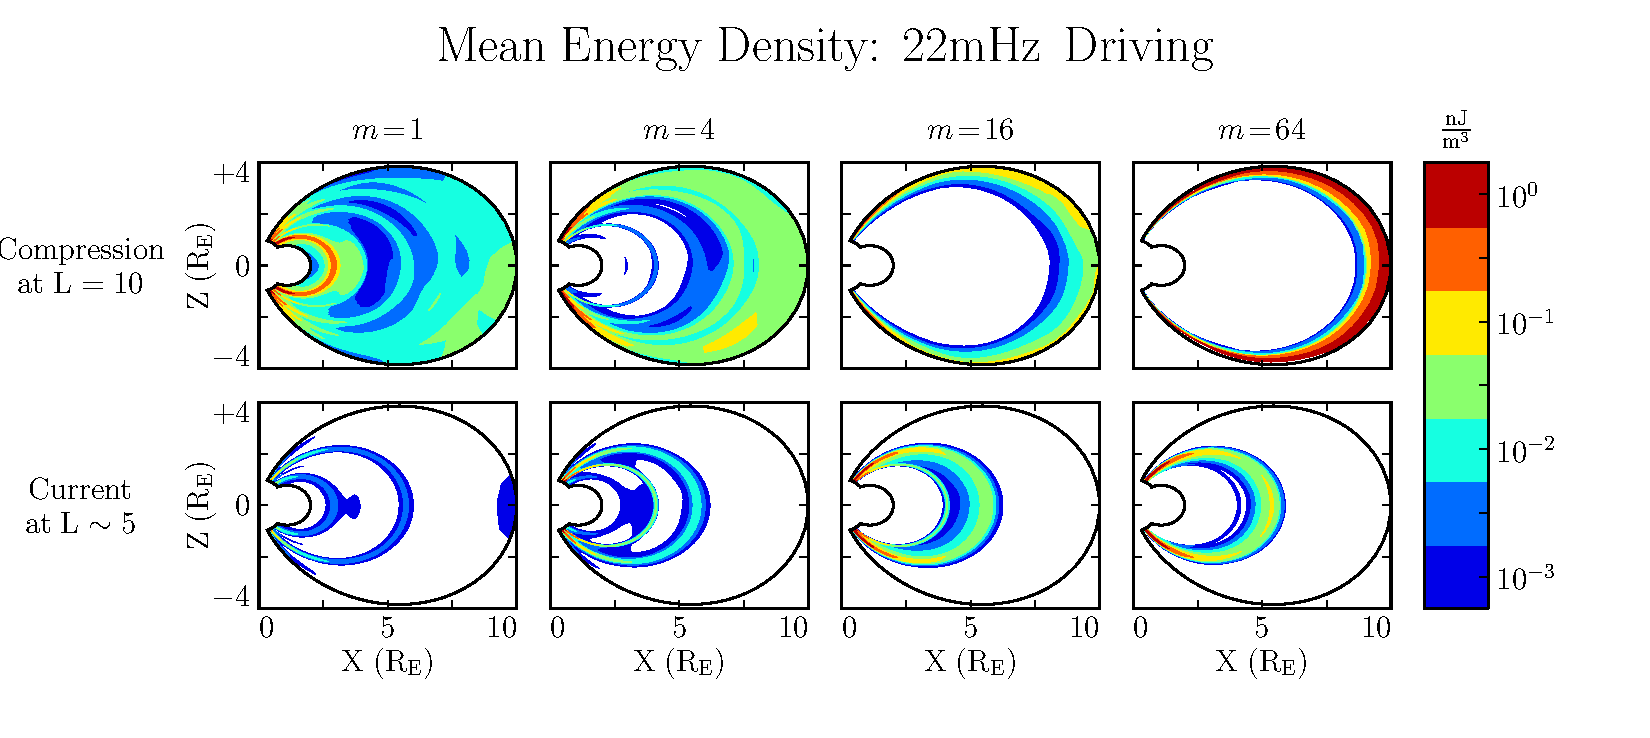
\includegraphics[width=\textwidth]{figures/drivers.pdf}%

\end{frame}

% -----------------------------------------------------------------------------
% -----------------------------------------------------------------------------
% -----------------------------------------------------------------------------

\begin{frame}
\frametitle{Maxwell's Equations}

Magnetic fields are updated using \farlaw:
\begin{align*}
  \tfrac{\partial}{\partial t} \vec{B} &= -\curl{E} &
  & \text{so} &
  &\highlight{ \vec{B} \assign \vec{B} - \dt \, \curl{E} }
\end{align*}

Electric fields are updated using \amplaw and \ohmlaw:
\begin{align*}
  \tensor{\epsilon} \cdot \tfrac{\partial}{\partial t} \vec{E} = \tfrac{1}{\mz} \curl{B} - \vec{J} - \tensor{\sigma} \cdot \vec{E}
\end{align*}

Let $ \quad \tensor{V}^2 \equiv \frac{1}{\mz} \tensor{\epsilon}^{-1} \quad $ and $ \quad \tensor{\Omega} \equiv \tensor{\epsilon}^{-1} \cdot \tensor{\sigma} \quad $ so
\begin{align*}
  \lr{ \tensor{\Omega} + \tensor{ \mathbb{I} } \tfrac{\partial}{\partial t} } \cdot \vec{E} &= \tensor{V}^2 \cdot \big( \curl{B} - \mz \vec{J} \big)
\end{align*}

Which can be solved with an integrating factor: 
\begin{gather*}
  \highlight{\vec{E} \assign \exp \arg{ -\tensor{\Omega} \, \dt } \cdot \vec{E} +
    \dt \, \exp \arg{ -\tensor{\Omega} \, \tfrac{\dt}{2} } \cdot
    \tensor{V}^2 \cdot \big( \curl{B} - \mz \vec{J} \big)}
\end{gather*}

\end{frame}

% -----------------------------------------------------------------------------
% -----------------------------------------------------------------------------
% -----------------------------------------------------------------------------

\begin{frame}
\frametitle{Coupling to the Atmosphere}

\begin{wideitemize}
\item Assume a perfectly-insulating atmosphere: $\curl{B} = 0$.  
\item From Maxwell's equations, $\div{B} = 0$. 
\item Then $\nabla^2\Psi = 0$ where $\nabla \Psi = \vec{B}$. 
\item Solution at the top of the atmosphere is a boundary condition:
\begin{align*}
  \tensor{\Sigma} \cdot \vec{E} &= \frac{1}{\mz} \,
    \displaystyle\lim_{\dr \rightarrow 0} \, \bigg[ \, \hat{r} \times \vec{B}
    \, \bigg|^{R_I + \dr}_{R_I - \dr}
\end{align*}
\item Solution at the bottom of the atmosphere gives ground signatures. 
\end{wideitemize}

\end{frame}

% =============================================================================
% ===================================================================== Results
% =============================================================================

\section{Numerical Results}

% -----------------------------------------------------------------------------
% -----------------------------------------------------------------------------
% -----------------------------------------------------------------------------

\begin{frame}
\frametitle{Snapshots of a Low-\azm Run}

\begin{columns}
\column{0.33\textwidth}
\begin{wideitemize}
\item Poloidal and compressional waves are blobby. 
\item Toroidal waves are sharply defined. 
\item All components are similar in magnitude. 
\end{wideitemize}
\column{0.67\textwidth}
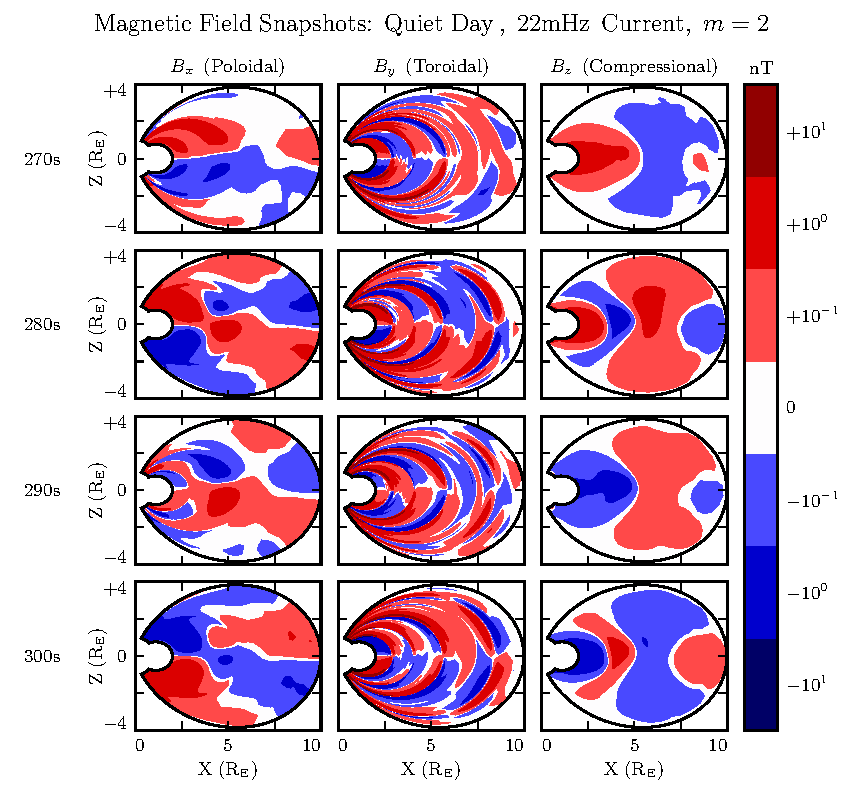
\includegraphics[width=\textwidth]{figures/snapshot_smallm.pdf}
\end{columns}

\end{frame}

% -----------------------------------------------------------------------------
% -----------------------------------------------------------------------------
% -----------------------------------------------------------------------------

\begin{frame}
\frametitle{Snapshots of a High-\azm Run}

\begin{columns}
\column{0.33\textwidth}
\begin{wideitemize}
\item Compressional field is weak. 
\item Little energy crosses field lines. 
\item Toroidal waves still sharper than poloidal ones. 
\end{wideitemize}
\column{0.67\textwidth}
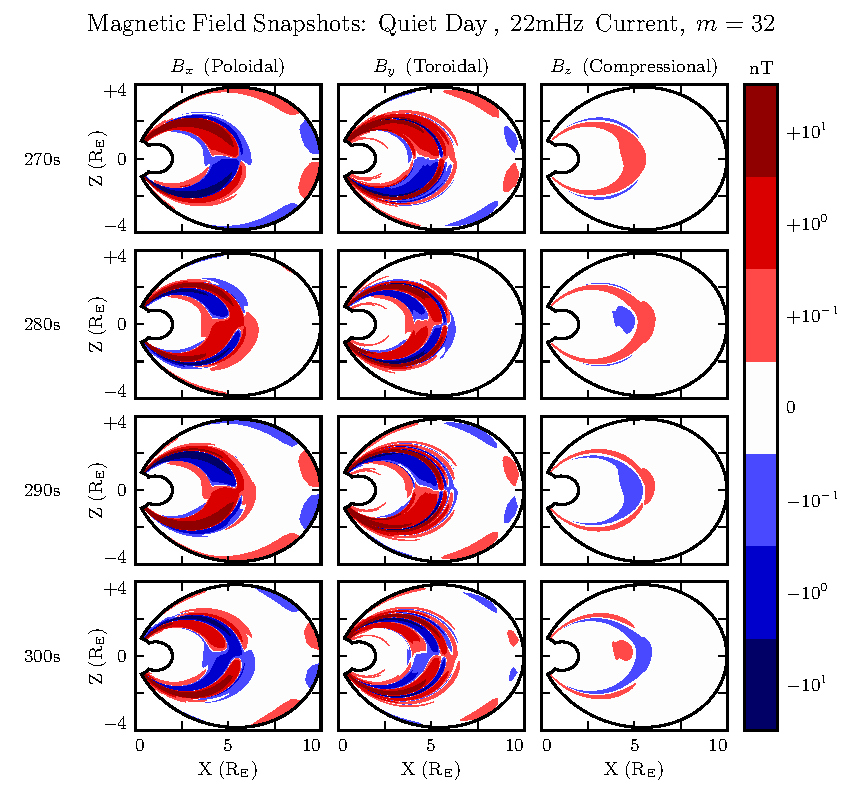
\includegraphics[width=\textwidth]{figures/snapshot_bigm.pdf}
\end{columns}

\end{frame}

% -----------------------------------------------------------------------------
% -----------------------------------------------------------------------------
% -----------------------------------------------------------------------------

\begin{frame}
\frametitle{Poloidal-to-Toroidal Rotation}

\begin{columns}
\column{0.33\textwidth}
\begin{overpic}[width=\textwidth]{figures/mann_1995.png}
 \put (0, 1) {\tiny\textcolor{black}{\;Mann and Wright, 1995}}
\end{overpic}%
\column{0.67\textwidth}
\begin{wideitemize}
\item Polarization rotates over time from poloidal to toroidal. 
\item The rotation is slower at large \azm. 
\item Toroidal FLRs do not rotate back. 
\end{wideitemize}
\end{columns}

\end{frame}

% -----------------------------------------------------------------------------
% -----------------------------------------------------------------------------
% -----------------------------------------------------------------------------

\begin{frame}
\frametitle{Resonance and Rotation on the Dayside}

\vfill 

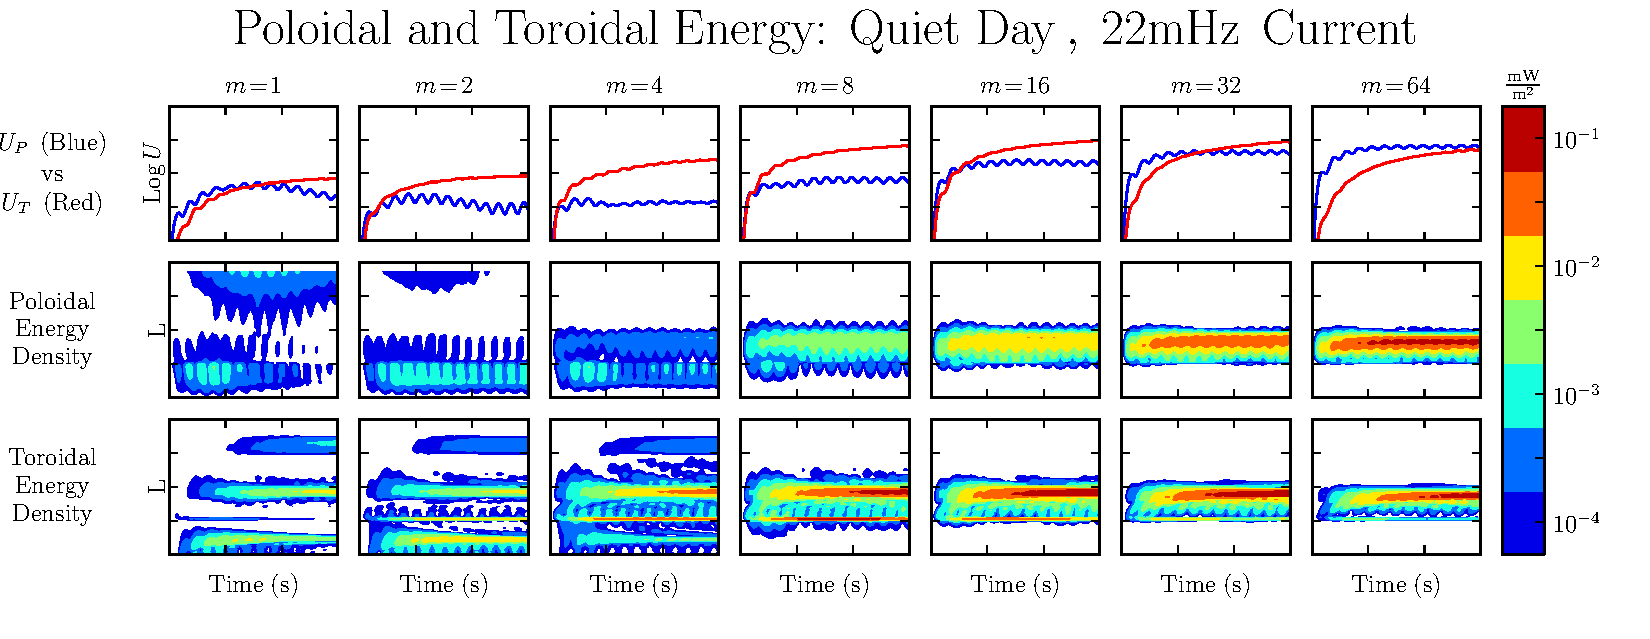
\includegraphics[width=\textwidth]{figures/energy_day.pdf}

\begin{wideitemize}
\item Poloidal-to-toroidal rotation timescales are comparable to the oscillation period, clearly faster than dissipation. 
% slowest at high \azm, toroidal asymptotically exceeds poloidal
%\item Toroidal energy asymptotically exceeds poloidal energy.
\item Toroidal energy accumulates only where resonant. 
\item At small \azm, energy escapes to the outer boundary. 
\end{wideitemize}

\end{frame}

% -----------------------------------------------------------------------------
% -----------------------------------------------------------------------------
% -----------------------------------------------------------------------------

\begin{frame}
\frametitle{Resonance and Rotation on the Nightside}

\vfill

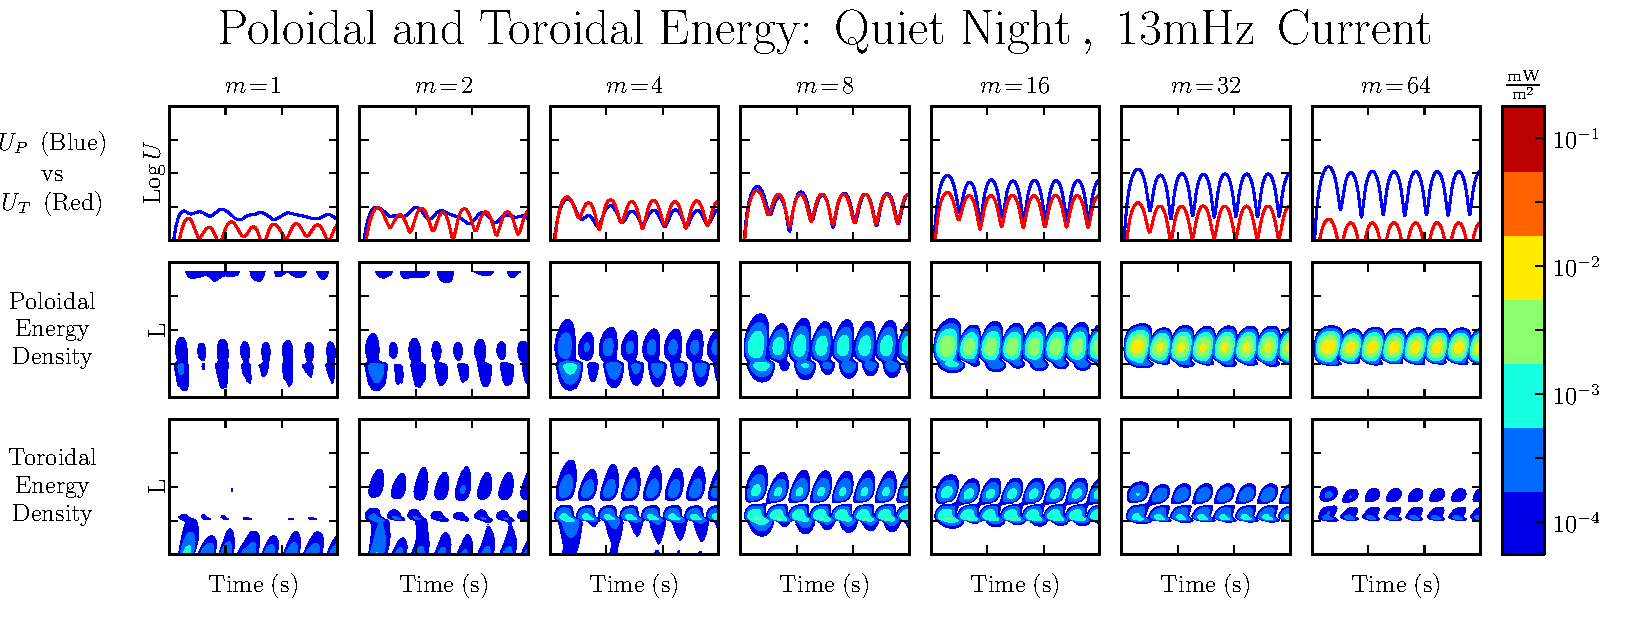
\includegraphics[width=\textwidth]{figures/energy_night.pdf}

\begin{wideitemize}
\item The nightside ionosphere is much less conductive than the dayside. 
\item No accumulation of energy over multiple drive periods. 
\item At high \azm, dissipation is faster than poloidal-to-toroidal rotation. 
\end{wideitemize}

\end{frame}

% -----------------------------------------------------------------------------
% -----------------------------------------------------------------------------
% -----------------------------------------------------------------------------

\begin{frame}
\frametitle{Ground Signatures and Giant Pulsations}

\begin{wideitemize}
\item Peak is in $B_\phi$, quiet conditions, \azm=16 to 32, \about\SI{65}{\degree} latitude. 
\item Counterclockwise at low latitude, clockwise at high latitude. 
\item It seems these properties are not unique to giant pulsations! 
\end{wideitemize}

\vfill

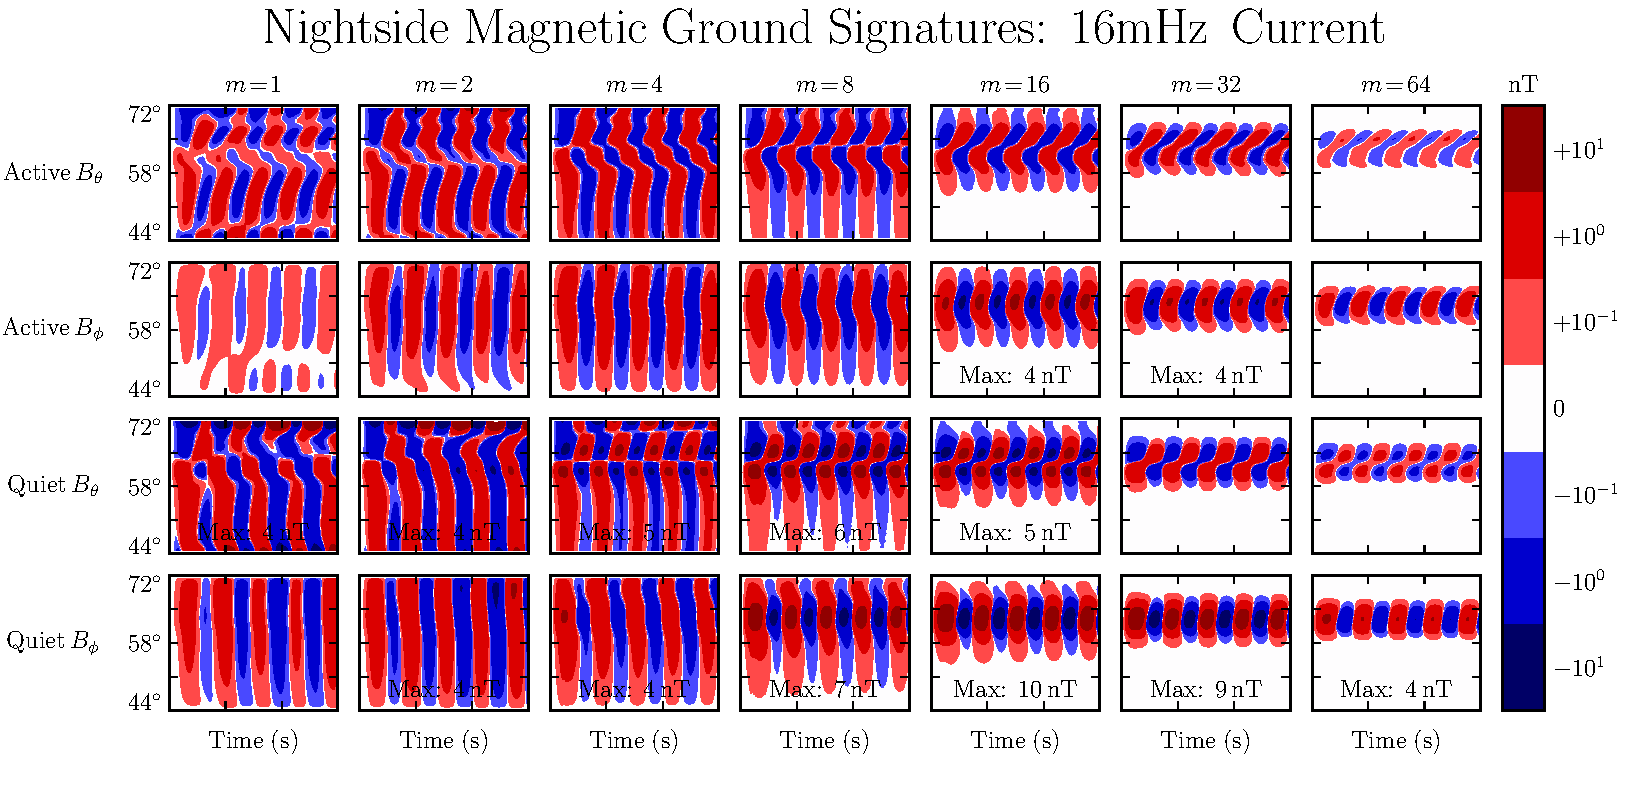
\includegraphics[width=\textwidth]{figures/ground_night.pdf}%

\end{frame}

% -----------------------------------------------------------------------------
% -----------------------------------------------------------------------------
% -----------------------------------------------------------------------------

\begin{frame}
\frametitle{Comparison to Observational Data?}

\begin{wideitemize}
\item How does the spatial distribution of giant pulsations compare to that of odd poloidal Pc4s?
\item How does the spatial distribution of odd toroidal Pc4s compare to that of odd poloidal Pc4s?
\item How about even toroidal and even poloidal Pc4s?
\item Past surveys do not address these questions.  
\end{wideitemize}

\end{frame}

% =============================================================================
% ======================================================================== RBSP
% =============================================================================

\section{Van Allen Probe Observations}

% -----------------------------------------------------------------------------
% -----------------------------------------------------------------------------
% -----------------------------------------------------------------------------

\begin{frame}
\frametitle{Distribution of Usable Data}


\begin{columns}
\column{0.33\textwidth}
\begin{wideitemize}
\item Data spans October 2012 to August 2015. 
\item Nightside has been sampled twice at apogee. 
\item Full 3D fields computed per $\vec{E} \cdot \vec{B} = 0$, about half the data gets tossed.
\end{wideitemize}
\column{0.67\textwidth}
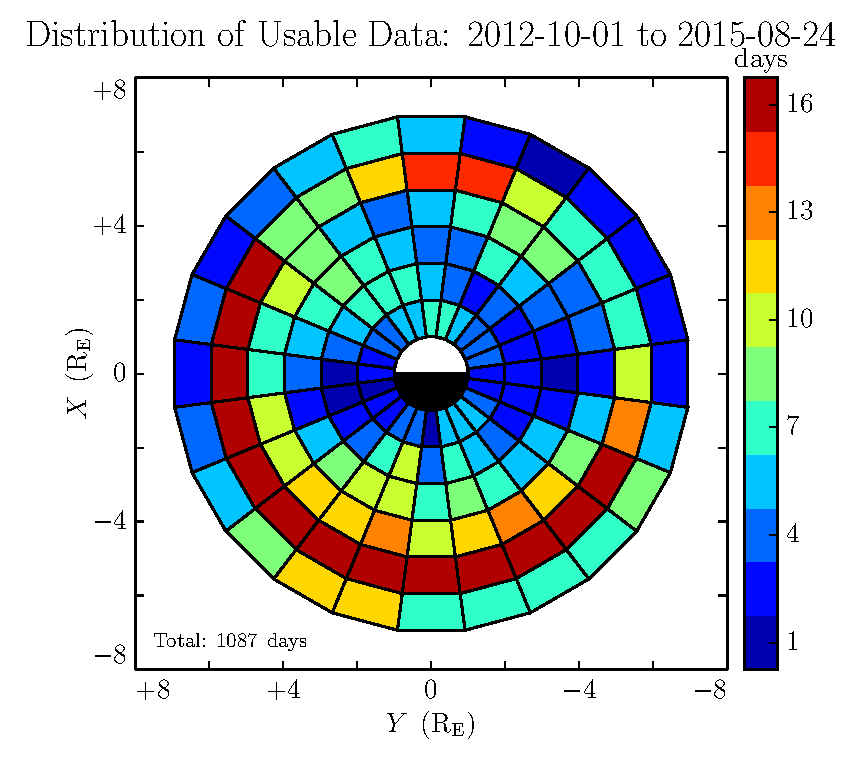
\includegraphics[width=\textwidth]{figures/pos_all_sharp.pdf}
\end{columns}

\end{frame}

% -----------------------------------------------------------------------------
% -----------------------------------------------------------------------------
% -----------------------------------------------------------------------------

\begin{frame}
\frametitle{Event Selection}

\begin{columns}
\column{0.5\textwidth}
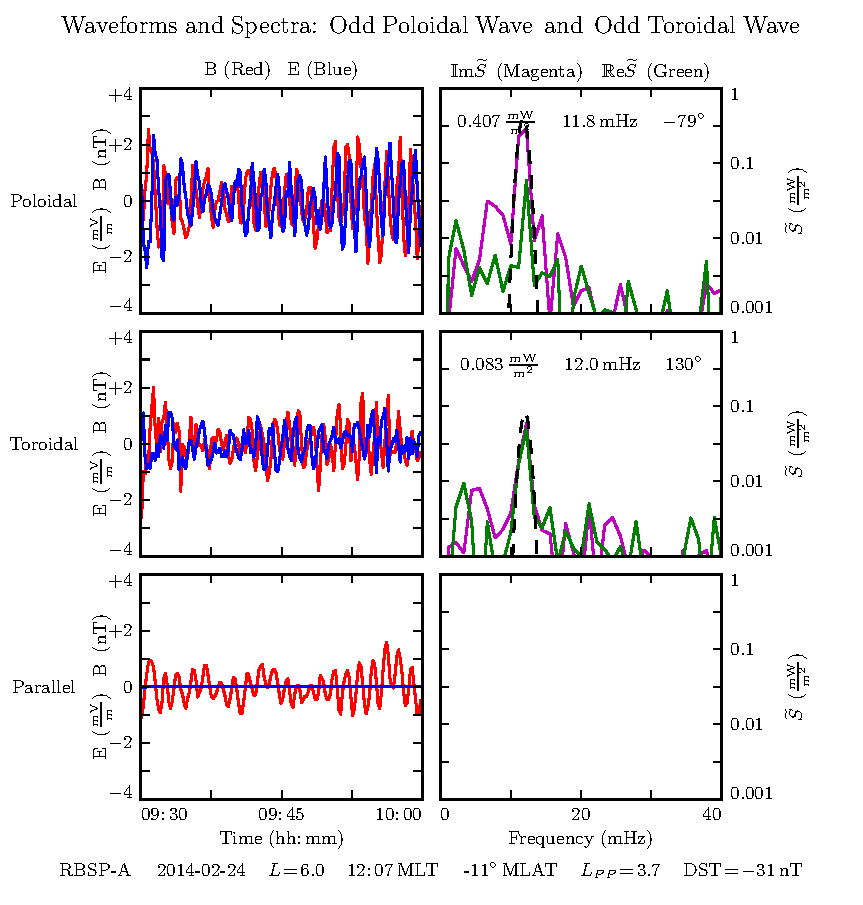
\includegraphics[width=\textwidth]{figures/sample_event_phase.pdf}
\column{0.5\textwidth}
\begin{wideitemize}
\item Split \about1000 days of data into half-hour events. 
\item Compute Poynting flux spectrum, effective at the ionosphere. 
\item Threshold on frequency, magnitude, coherence, and spectral width. 
\item Characterize each event by polarization and harmonic. 
\end{wideitemize}
\end{columns}

\end{frame}

% -----------------------------------------------------------------------------
% -----------------------------------------------------------------------------
% -----------------------------------------------------------------------------

\begin{frame}
\frametitle{Pc4 Observation Rate}

\begin{columns}
\column{0.33\textwidth}
\begin{wideitemize}
\item Peak observation rate at noon.  
\item Fewest events at dusk. 
\item Stragglers near midnight. 
\item Generally consistent with previous surveys of Pc4 events. 
\end{wideitemize}
\column{0.67\textwidth}
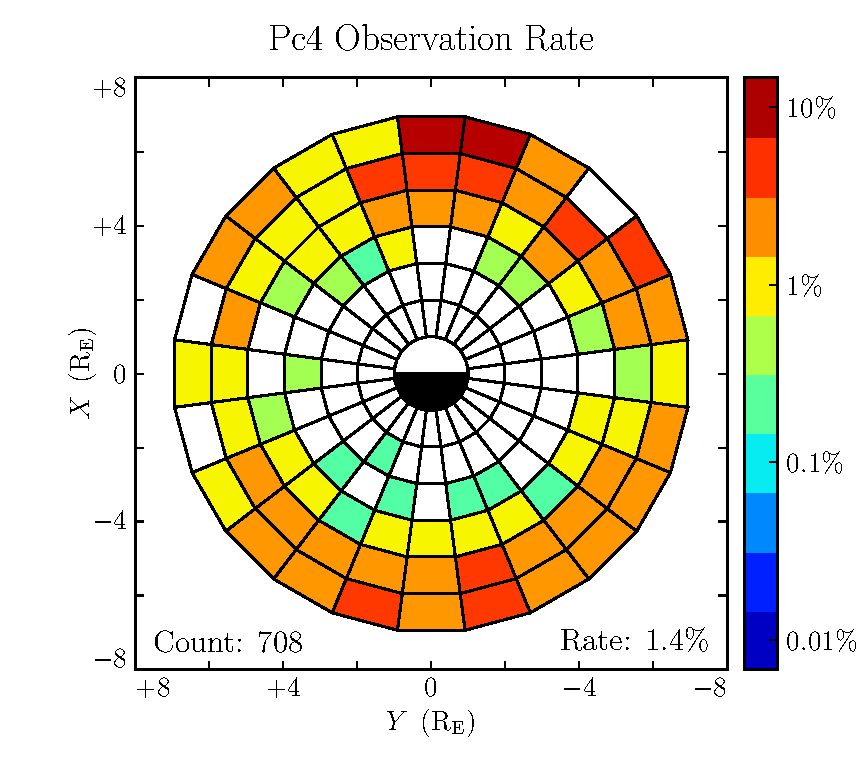
\includegraphics[width=\textwidth]{figures/rate_all_sharp.pdf}
\end{columns}

\end{frame}

% -----------------------------------------------------------------------------
% -----------------------------------------------------------------------------
% -----------------------------------------------------------------------------

\begin{frame}
\frametitle{Pc4 Observation Rate by Mode}

\begin{columns}
\column{0.33\textwidth}
Questions from before:

\vspace{5pt}

\begin{wideitemize}
\item Where are odd poloidal Pc4s compared to giant pulsations?
\item Where are odd toroidal Pc4s compared to odd poloidal Pc4s?
\item How about even toroidal and even poloidal Pc4s?
\end{wideitemize}
\column{0.67\textwidth}
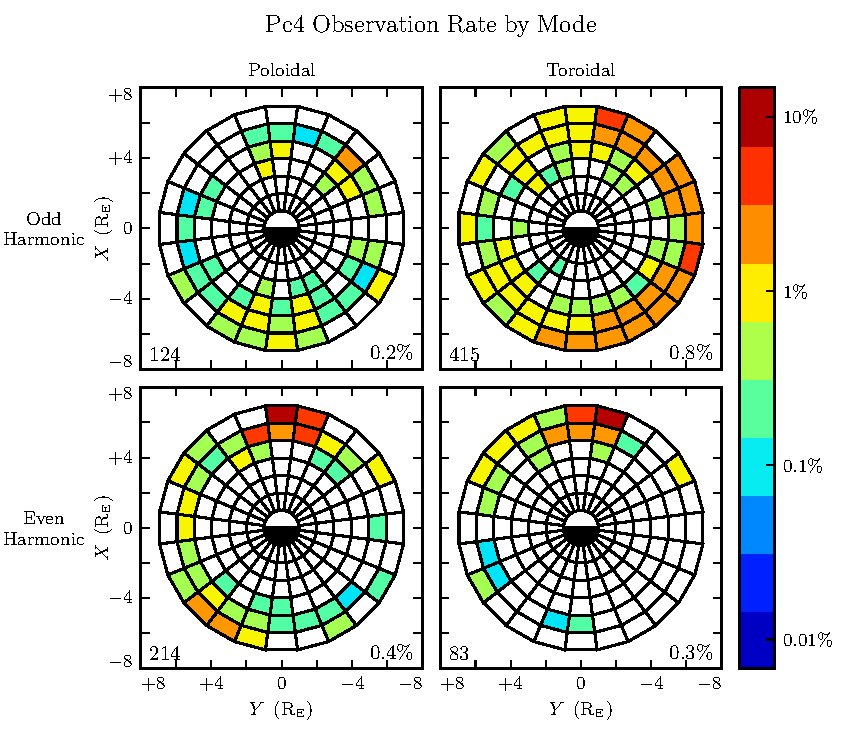
\includegraphics[width=\textwidth]{figures/mode_all_sharp.pdf}
\end{columns}

\end{frame}

% -----------------------------------------------------------------------------
% -----------------------------------------------------------------------------
% -----------------------------------------------------------------------------

\begin{frame}
\frametitle{Phase Distribution of Pc4 Events}

\begin{wideitemize}
\item Estimate wave lifetime from characteristic values $B$, $E$, and $R$:
\begin{align*}
  \tau &= \frac{BR}{2 E \cos\varphi} &
  & \text{where} &
  \varphi \equiv \arctan\frac{ \imag\dft{S} }{ \real\dft{S} }
\end{align*}
\item Standing waves: $\varphi = \pm\SI{90}{\degree}$. Traveling waves: $\varphi = \SI{0}{\degree}$ or \SI{180}{\degree}. 
\item Odd modes are spread more from $\pm\SI{90}{\degree}$, at least at the equator. 
\end{wideitemize}

\vfill

\centerline{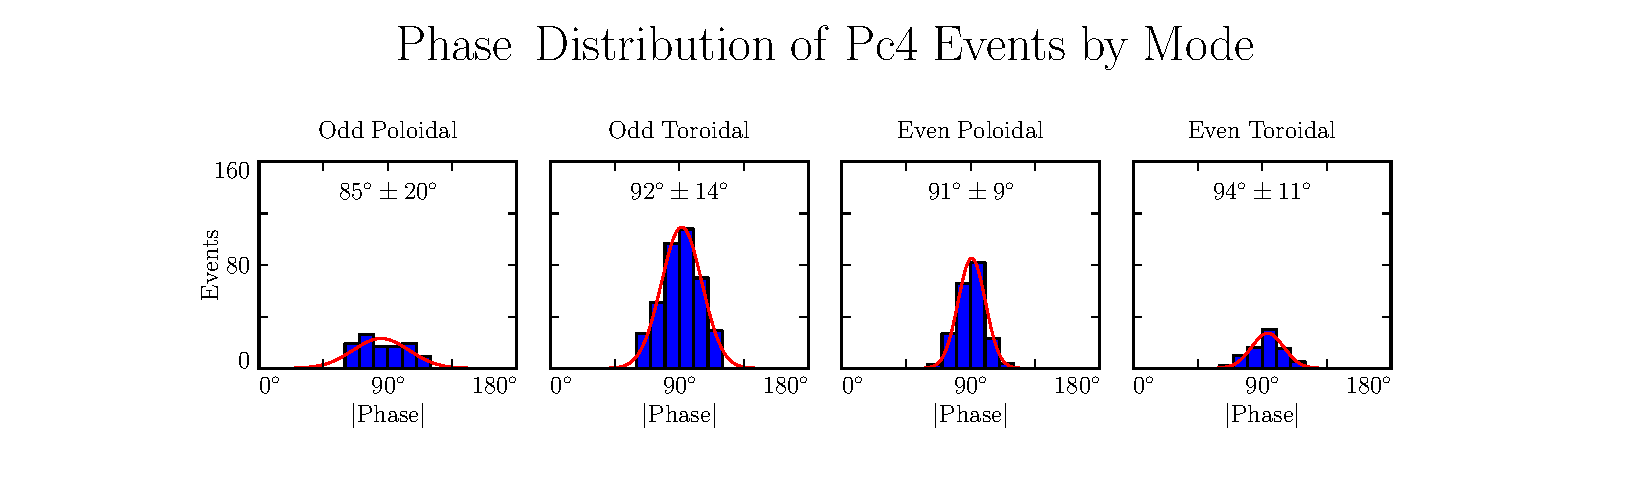
\includegraphics[width=1.2\textwidth]{figures/phase_across.pdf}}

\end{frame}

% =============================================================================
% ================================================================== Conclusion
% =============================================================================

\section{Conclusion}

% -----------------------------------------------------------------------------
% -----------------------------------------------------------------------------
% -----------------------------------------------------------------------------

\begin{frame}
\frametitle{Summary}

\begin{wideitemize}
\item Pc4s and giant pulsations are known to have a mishmash of heretofore-unrelated properties. 
\item Tuna is a new model designed with Pc4s in mind. 
\item Numerical results suggest several novel relationships between Pc4 properties. 
\item Van Allen Probe survey supports numerical results, and poses new questions. 
\end{wideitemize}

\end{frame}

% -----------------------------------------------------------------------------
% -----------------------------------------------------------------------------
% -----------------------------------------------------------------------------

\begin{frame}
\frametitle{Acknowledgements}

\begin{columns}
\column{0.33\textwidth}
Committee:
\column{0.34\textwidth}
Funding:
\column{0.33\textwidth}
Collaborators:
\end{columns}

\begin{columns}
\column{0.33\textwidth}
\begin{wideitemize}
\item Bob Lysak (Advisor)
\item Cindy Cattell (Chair)
\item Tom Jones
\item Lindsay Glesener
\end{wideitemize}
\column{0.34\textwidth}
\begin{wideitemize}
\item NSF grant AGS-1405383
\item UMN OVPR
\item NASA grant NNX12AD14G
\item GEM Student Support
\end{wideitemize}
\column{0.33\textwidth}
\begin{wideitemize}
\item John Wygant
\item Lei Dai
\item Ian Mann
\item Aaron Breneman
\item Scott Thaller
\item Sheng Tian
\end{wideitemize}
\end{columns}

\end{frame}

% =============================================================================
% =============================================================== Backup Slides
% =============================================================================

\backupbegin
\section{Backup Slides}

% -----------------------------------------------------------------------------
% -----------------------------------------------------------------------------
% -----------------------------------------------------------------------------

\begin{frame}
\frametitle{Summary}

\end{frame}

% =============================================================================
% ================================================================ End Document
% =============================================================================

\backupend

\end{document}



